Um einen Eindruck zur Beliebtheit von PoW-basierten Kryptowährungen im Vergleich zu PoS-basierten zu erhalten, ist die Marktkapitalisierung eine aussagekräftige Kennzahl. Die am Markt erfolgreichsten Kryptowährungen für PoW und PoS  sind online auffindbar\citebib{coinmarket2}{}{vgl. }:
\FloatBarrier
\begin{figure}[ht!]
    \centering
    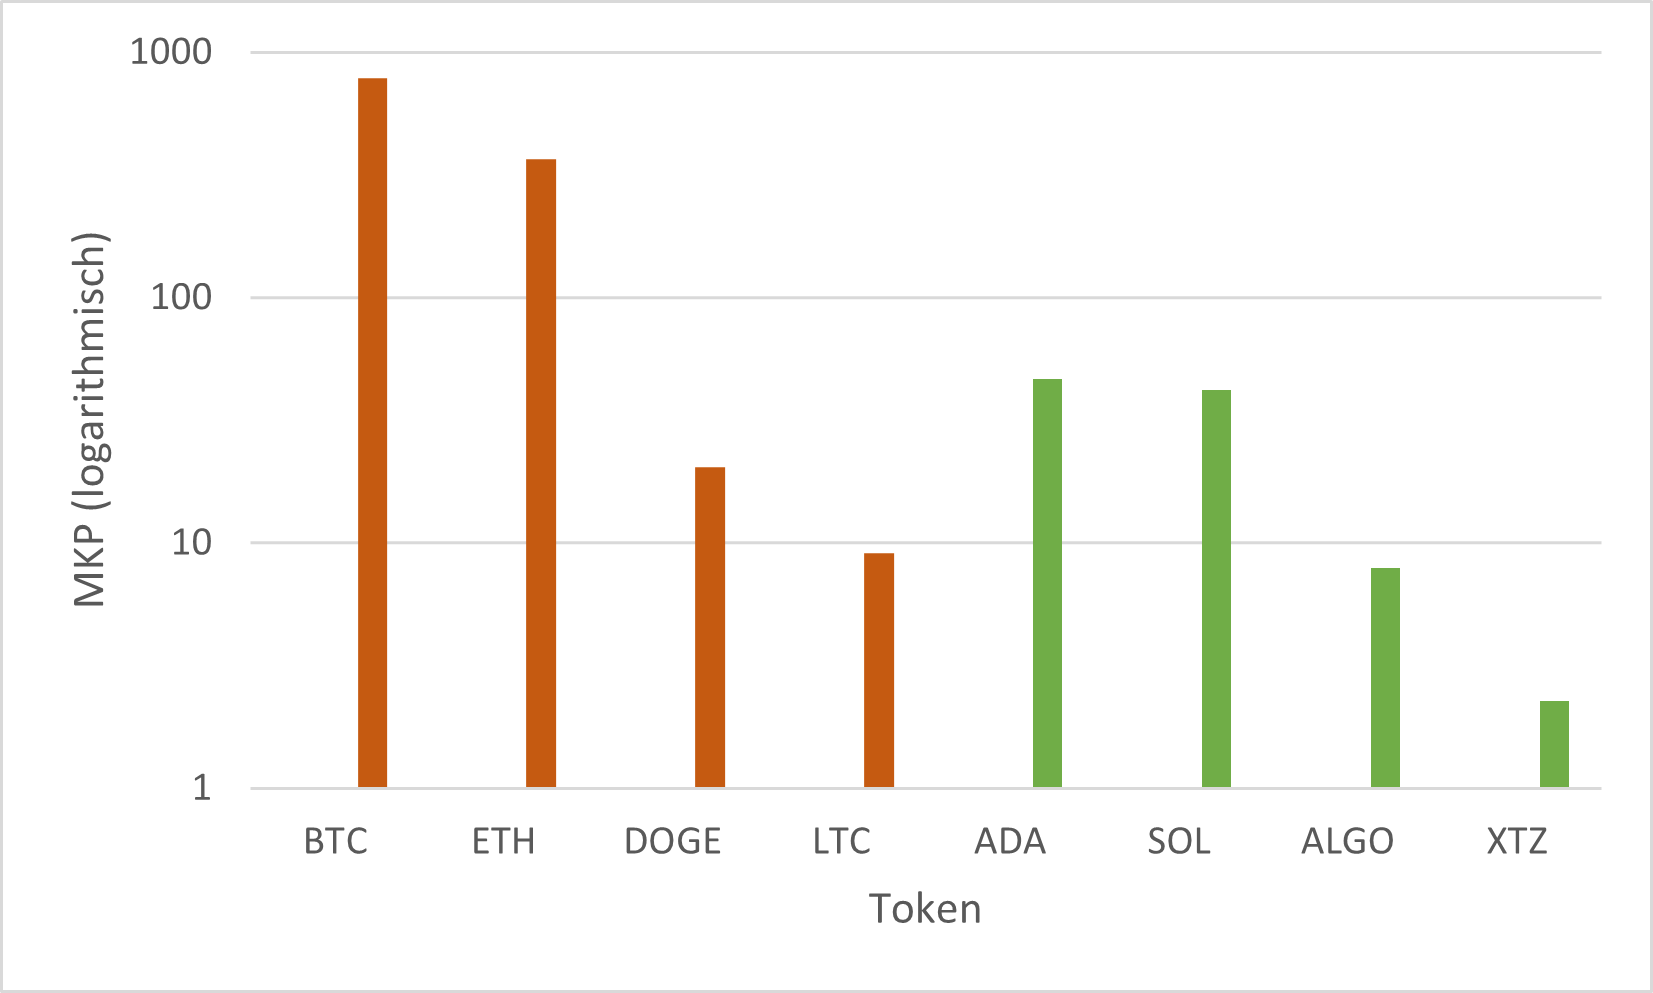
\includegraphics[width=.75\textwidth]{quellen/mkp_pow_pos.png}
    \caption{Vergleich Marktanteil von PoW- und PoS-Netzwerken 2022}
\end{figure}
\FloatBarrier
\noindent Wie zu erkennen ist, haben die beiden PoW-Tokens Bitcoin und Ethereum den größten Marktanteil. Allerdings verzeichnen PoS-Tokens, wie Cardano oder Solana über das letzte Jahr verteilt eine stetig anwachsende Marktkapitalisierung, während der Kurs der PoW-Tokens im Vergleich dazu stagniert.\citebib{coinmarket2}{}{vgl. }. Diese Entwicklung könnte darauf hindeuten, dass die energiesparenden PoS-Tokens in der Öffentlichkeit deutlich an Zuspruch gewinnen. Dies könnte ein weiterer ausschlaggebender Punkt dafür sein, dass Netzwerke wie Ethereum trotz ihrer hohen Marktkapitalisierung auf PoS umsteigen.